% LaTeX .tex
% Example for the proceedings of the  25th International Congress of Mechanical Engineering
% COBEM 2019
% October, 20-25, 2019, Uberlândia, MG, Brazil
% Based on the template of the proceedings of COBEM2015 and COBEM2017

\documentclass[10pt,fleqn,a4paper,twoside]{article}
\usepackage{abcm}
\def\shortauthor{F. J. O. Ribeiro, I. A. Macedo, R. L. R. Neves and R. P. Reis}
\def\shorttitle{Development and Validation of Winding Machine}
\usepackage{blindtext}
\usepackage{subcaption}
\begin{document}
\fphead
\hspace*{-2.5mm}\begin{tabular}{||p{\textwidth}}
\begin{center}
\vspace{-4mm}
\title{DEVELOPMENT AND VALIDATION OF EPOXY REINFORCED GLASS-FIBER FILAMENT WINDING MACHINE}
\end{center}
\authors{Felipe Jos\'{e} Oliveira Riberio} \\
\authors{Izaaque Aniceto Macedo} \\
\institution{Federal University of Uberlândia (UFU), Av. João Naves de Ávila, 2121, Campos Santa Mônica, Uberlândia, MG } \\
\institution{feliperibeiro.ufu@gmail.com} \\
\institution{izaaque@live.com} \\
\authors{Rodrigo Lira Reis Neves} \\
\authors{Ruham Pablo Reis} \\
\institution{Federal University of Uberlândia (UFU), Av. João Naves de Ávila, 2121, Campos Santa Mônica, Uberlândia, MG } \\
\institution{rodrigolira1999@gmail.com} \\
\institution{ruhamreis@ufu.br} \\
\\
\abstract{\textbf{Abstract.} In the present paper, the construction and validation of a low-cost automated composite filament winding machine is discussed. Such mechanism can apply wet polymeric fiber filaments, after a resin bath, to a rotating mandrel, in a precise and regular manner. Such configuration is very used in the industry for being the most cost-effective and reliable method for creating very resilient and uniform cylindrical structures. This is an initiative of the Propulsion and Aerospace Technology Team (EPTA) that will make possible the manufacturing of fuselages for high Mach rocketry. In these regards, all the design, construction and validation processes will be addressed.}\\
\\
\keywords{\textbf{Keywords:} Winding machine, composite materials, Glass-fiber reinforced epoxy, aerospace structure, automation.}\\
\end{tabular}

\section{INTRODUCTION}


Fiber-reinforced polymeric materials have been successfully replacing metallic mechanical parts in all sorts of structures, from glass fiber pipes to the graphite fiber composite wing sections of the F-18 fighter jet \citep{vari_bobi}. The composite materials are becoming the standard in all sorts of engineering applications. Such fact is due to its very singular properties of high stress resistance for a low weight \citep{bobinamento}, which makes this material specially applicable to aerospace engineering.
But, although the advantages, there is some problems. The non homogeneity of the material makes its application difficult as the qualities on the part normally deviate from the averaged properties \citep{utilizacaoi}. The composite materials are anisotropic too, which further complicates whatever mechanical application it is used.      

In the composite industry, the process of filament winding has gaining popularity, as it is the most cost effective method for producing pressure retaining structures reinforced with polymeric fibers \citep{influence_tension}. Other feature of such process is the opportunity of simple automation, which results in precision and regularity in the final structure. This results in something that can be well applied in rocketry engineering, as the fuselage of these vehicles are cylindrical and have to resist to high compressive forces, and such reinforcement is critical to contain buckling \citep{rocket_tube}. 

In these regards, in the present paper the authors aim to develop an automated winding machine with two degrees of freedom for rocketry structural applications in the Propulsion and Aerospace Technology Team (EPTA). 
This machine should have low cost, but be sufficiently reliable for the proposed usage, being capable of making cylindrical fuselages up to 900 mm of length and 180 mm of diameter. The material intended to be used in the winding process is the epoxy reinforced glass-fiber. So, fused deposition modeling was applied to create almost all the structure and components of the machine. For the electronics, an Arduino UNO was used, with two step motors for both rotate the mandrel and move the winding carriage, resulting in an efficient and cost-effective configuration. 

Finally, after the design, some composite parts will be produced, tested and compared with literature \citep{ensaio_artigo} for validating the filament winding machine.





\section{MACHINE DESIGN}

The project dimensions were determined by the maximum geometry intended for production. Based on that, the main machine dimensions should encompass an useful winding length of $900$ mm and $180$ mm of maximum cylinder diameter. Thus this machine configuration layout is separated on the following modules:  The bench base, the mandrel supports, the winding carriage and the electronics control unit.

\subsection{MECHANICAL PARTS}

The machine should have two movable parts. First, the mandrel should be capable of rotating around its central axis (Fig.\ref{i4}.C). For that to happen, there has to be two supports with bearings. The distance between these supports define the overall length of the central structure. Secondly, the winding carriage has to move freely throughout all the cylinder length, so the bench base has to let such movement to happen (as seen in Fig.\ref{i4}.B).

The carriage must contain a device similar to eyelets aiding the fibers arrangement. It has a resin bath container and it is equipped with rollers to control the fibers passage. So the fiber comes from the glass-fiber coil (Fig.\ref{i4}.A), pass through the winding carrier were it is layered in resin and guided for the mandrel. The relationship between the velocity of the carrier and rotation of the coil determine the winding angle, a critical parameter for the resulting mechanical properties of the winded part. 

\begin{figure}[!h]
	\centering
	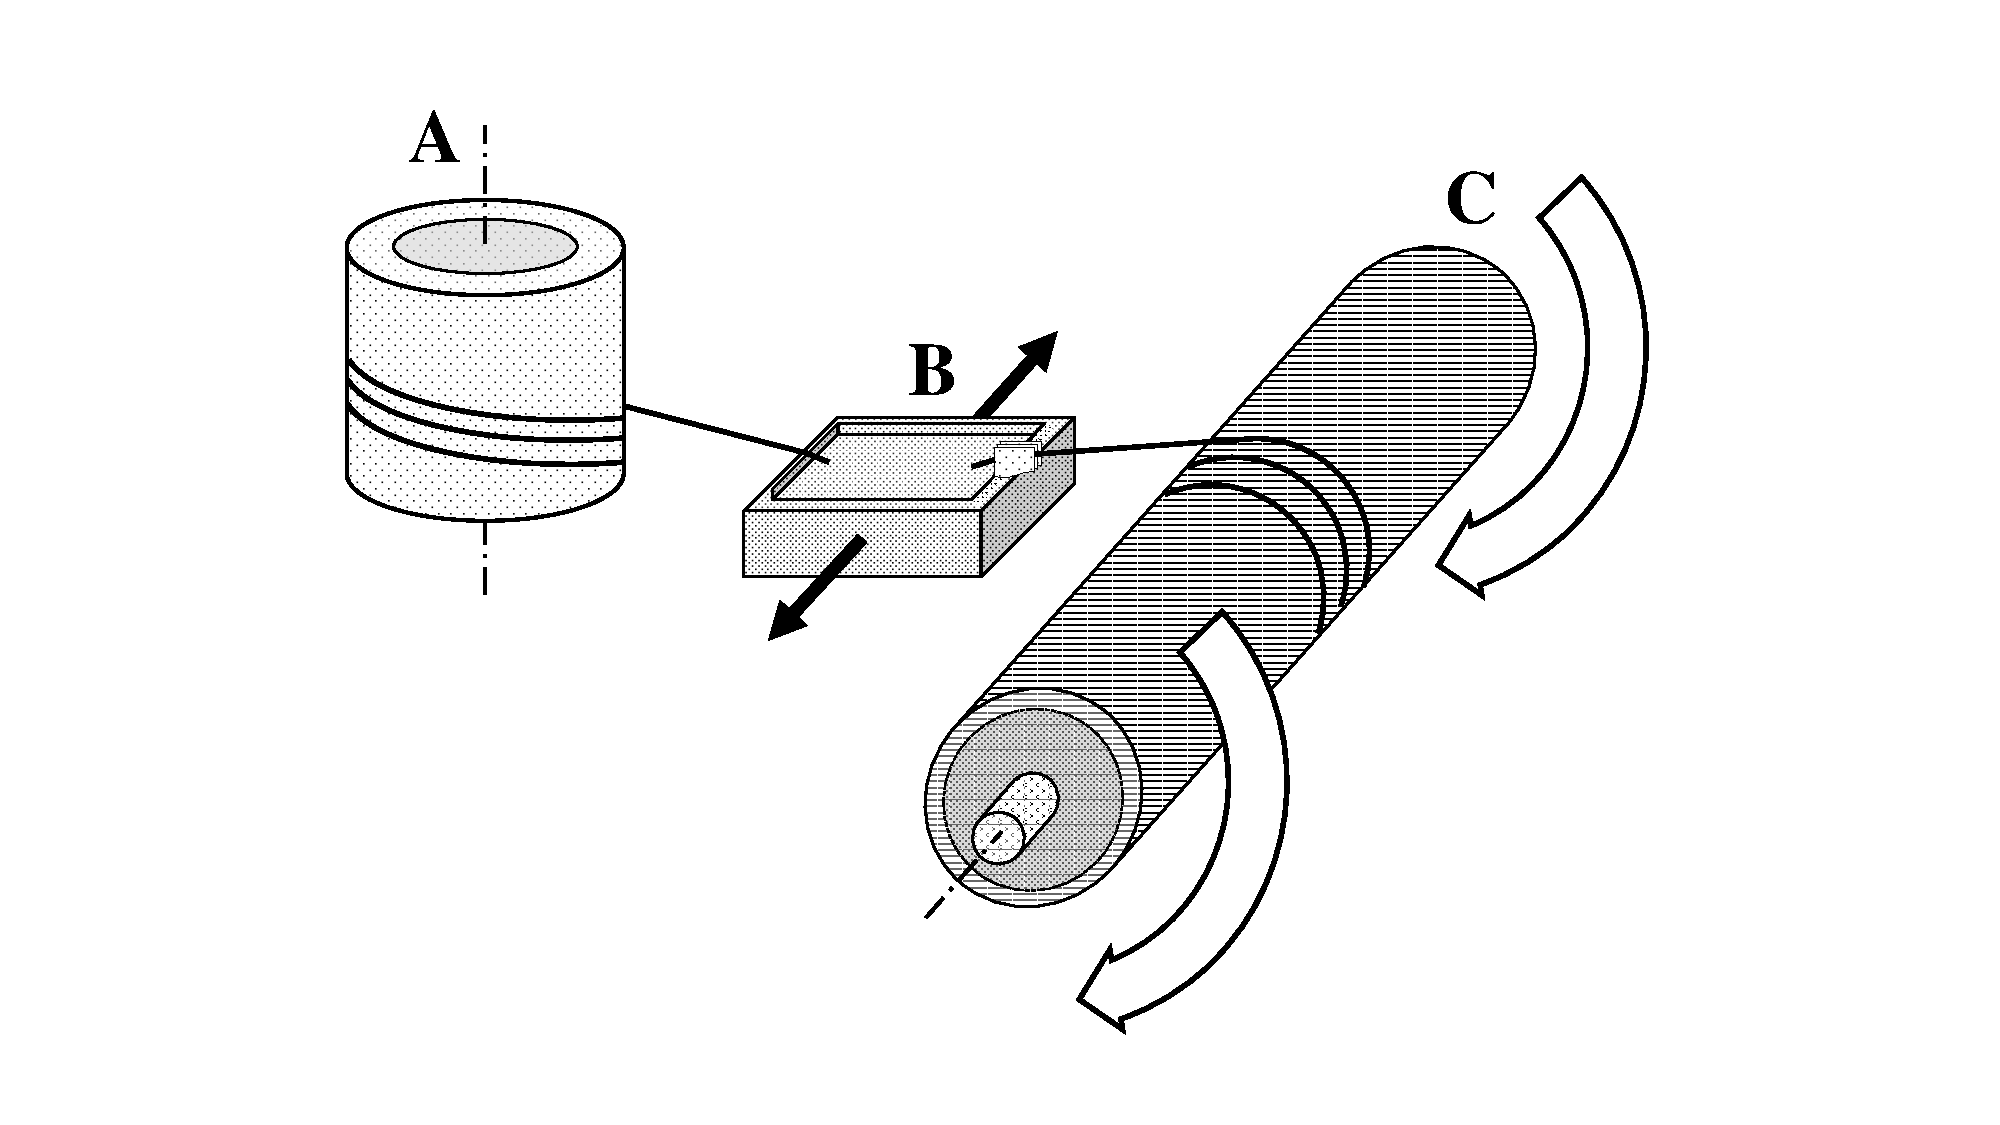
\includegraphics[angle=0, scale=0.45]{imagens/imagem1}
	\caption{Graphical representation of the filament winding machine.}
	\label{i4}
\end{figure}

To geometrically determine the central structure (bench base), the useful winding length was used. Besides this measure, it is necessary a relaxation zone, were the winding angle will not be respected. This relaxation zone is important in the moment that the carrier changes direction \citep{livro_prof} and normally it is cut off from the resulting piece. So, to calculate this relaxation zone, it is used the Equation.\ref{e1}:

\begin{equation}\label{e1}
\theta_{min} = arctg \left(\frac{b}{a}\right)
\end{equation}

Where $\theta_{min}$ is the minimum winding angle possible, $b$ is the distance between the eyelet and the center of the mandrel and $a$ is the relaxation zone. The minimum winding angle chosen for this machine was $33^\circ$, resulting in an relaxation zone of 150 mm.

Such fact resulted in an mandrel with a total length of 1200 mm. The structure was developed accordingly, with supports to accommodate such dimensions. The bench base was made even bigger, to let the carrier's eyelet reach the total extension of the mandrel.  



\begin{figure*}[!h]
\centering
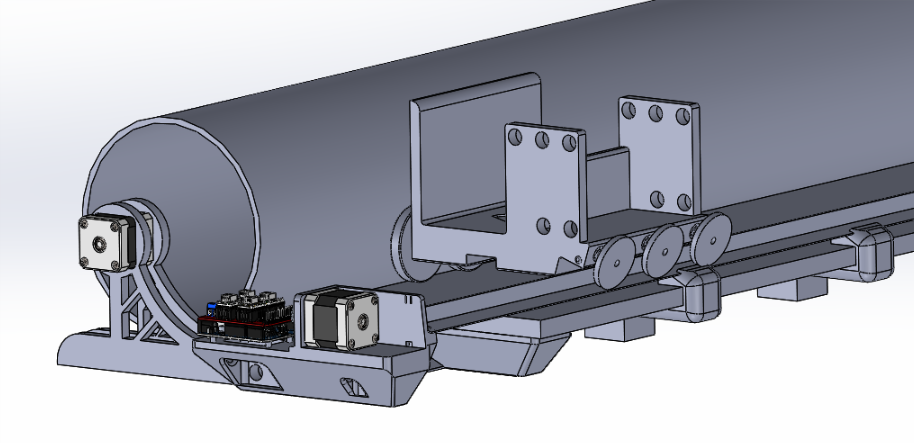
\includegraphics[angle=0, trim = {0mm 0mm 30mm 10mm}, clip , scale=0.3]{imagens/cad}
\caption{Solid Works model design.}
\label{i5}
\end{figure*}




\subsection{ELECTRONIC PARTS}

Now, with the structure defined, there must be the control of the moving parts. So, two step motors Nema 17 were chosen to drive the system. The first was placed in one of the supports that hold the mandrel and the second in the bench base, linked to a rubber belt fixed in the winding carrier (Fig.\ref{i5}).

It was chosen an Arduino UNO as the micro-controller of the systems, embedded with an CNC shield to aid with the DRV8825 drivers communication. A button was placed on the bench base to mark the beginning of the system to the controlling unity. The controlling unity components can be seen in Figure.\ref{i6}.


\begin{figure*}[!h]
	\centering
	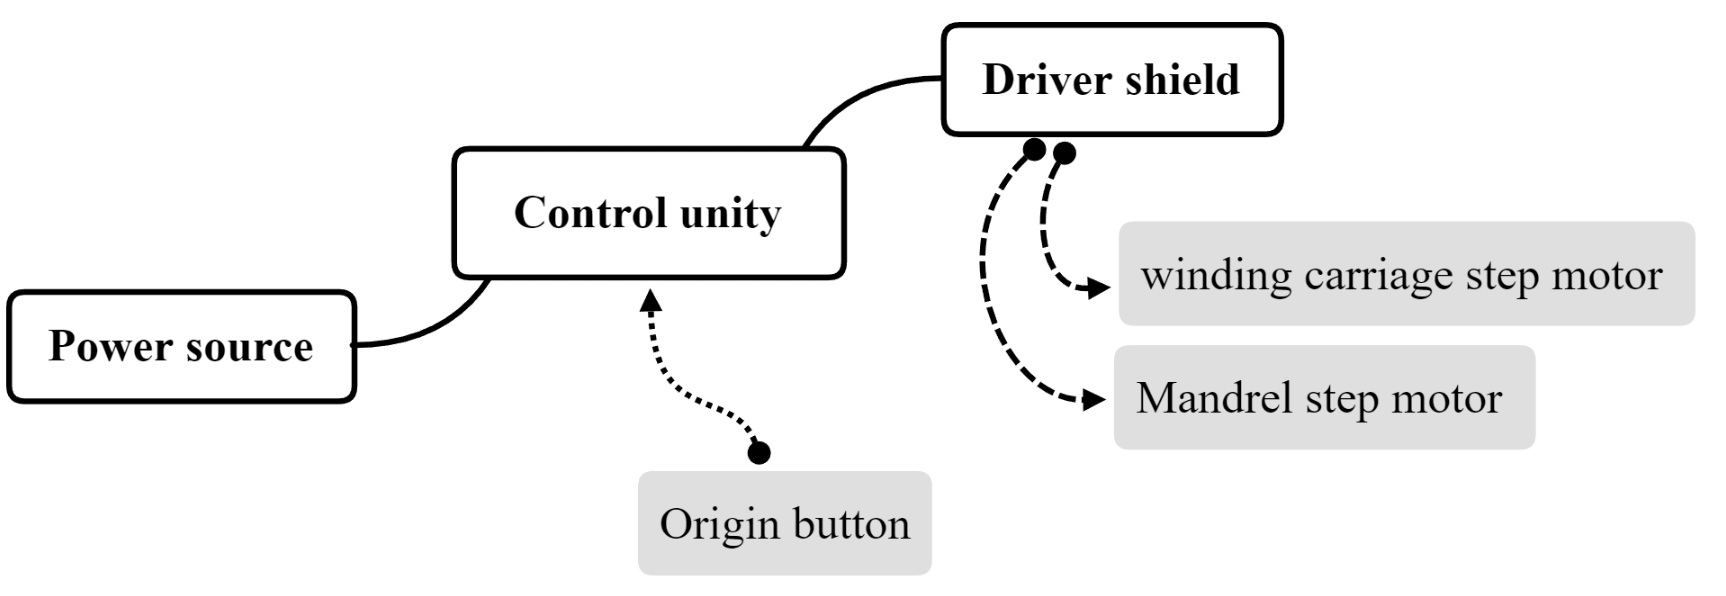
\includegraphics[angle=0, trim = {0mm 0mm 0mm 0mm}, clip , scale=0.25]{imagens/eletronic}
	\caption{Electronic scheme of the controlling unity.}
	\label{i6}
\end{figure*}

So, when the winding process is initiated, the first action of the machine is to move the carrier to the left until the button is pressed, and then initiating the rotation of the mandrel and the filamentation process.

The relationship between the winding angle and the velocities applied to the step  motors is defined ahead \citep{design_fiber}:   

\begin{equation}
\theta = \frac{2\pi r N_m}{V_c}
\end{equation}

Where $\theta$ is the winding angle, $r$ is the mandrel radius, $N_m$ is the mandrel rotation speed and $V_c$ is the carriage linear velocity.     





\section{MECHANISM VALIDATION}
For the mechanism validation, test parts will be made with the objective of comparing the mechanical properties with literature reference \citep{ensaio_artigo}. Such parts will be made accordingly with the ASTM D3039-76 standards \citep{astm}.

\begin{figure*}[!h]
	\centering
	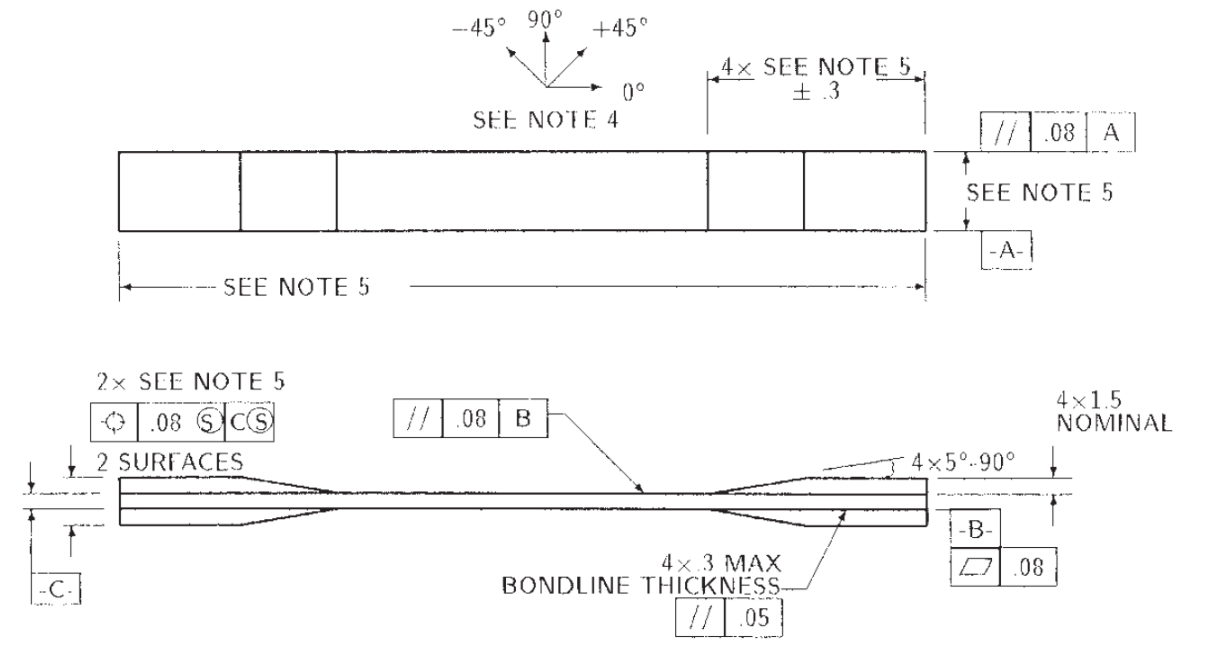
\includegraphics[angle=0, trim = {0mm 0mm 0mm 0mm}, clip , scale=0.5]{imagens/specimens}
	\caption{Specimens for mechanical test validation.}
	\label{i7}
\end{figure*}

The mechanical tests will be made and will be present in the final paper. The influence od factors such as winding angle and tension 
will be analyzed. The integration of the glass-fiber and the printed mold will be seen too, aiming to develop a hybrid structure (polymer and composite). In this case the influences of surface finish of the mold relative to the adhesion of the fiber to the mold will be discussed. The object is to apply such technology in the rockets fuselages made by the Propulsion and Aerospace Technology Team (EPTA).  

\section{CONCLUSION}

In the present paper the authors described the design of a low-cost automated polymer filament winding machine for aerospace applications, specifically to rockets. It was noticed how the 3D printing can make the building much cheaper, as the polymer needed for all the printed structures didn't surpassed more than 3 KG of PETG 3D printing resin. The Arduino make the design process much accessible too, because it simplifies the electronics and is a low-cost protoboard.   

For the final paper, the structural team fo the Propulsion and Aerospace Technology Team (EPTA) aim to further enhance the machinery in this paper developed, performing the mechanical tests previously described.  




\section{ACKNOWLEDGEMENTS}
The authors would like to thank the following institutions: LMEst (Structural Mechanics Laboratory), FEMEC (Mechanical engineering College), UFU (Federal University of Uberl\^andia) and, especially, EPTA(Propulsion and Aerospace Technology Team) for the financial and technical support.

\section{REFERENCES} 

\bibliographystyle{abcm}
\renewcommand{\refname}{}
\bibliography{bibfile}

\end{document}
